% Affirming Unattested Expertise at Ceiling Confidence (v2).
%
% No measured number is typed in this file. Each is a macro (\tiXxx) or a table/figure that
% scripts/export_paper_tables.py writes from results/*.json into paper/generated/.
% tests/test_paper.py rebuilds that output, requires it byte-identical to the committed copy,
% and refuses any decimal literal in this file that is not a generated value.
% arXiv: primary cs.IR or cs.CY, cross-list cs.CL, stat.AP.
\documentclass[11pt]{article}

\usepackage[margin=1in]{geometry}
\usepackage[T1]{fontenc}
\usepackage{lmodern}
\usepackage{booktabs}
\usepackage{tabularx}
\usepackage{pgfplots}
\pgfplotsset{compat=1.18}
\usepackage{amsmath}
\usepackage{microtype}
\usepackage{url}
\usepackage[font=footnotesize,skip=3pt]{caption}
\usepackage[hidelinks]{hyperref}
\usepackage[numbers,sort&compress]{natbib}

\setlength{\tabcolsep}{4pt}
\sloppy
\makeatletter
\renewcommand\paragraph{\@startsection{paragraph}{4}{\z@}%
  {1.4ex \@plus .4ex \@minus .2ex}{-1em}{\normalfont\normalsize\bfseries}}
\makeatother
\setlength{\textfloatsep}{9pt plus 2pt minus 2pt}
\setlength{\floatsep}{8pt plus 2pt minus 2pt}

% GENERATED by scripts/export_paper_tables.py from results/*.json. Do not edit.
\newcommand{\tiAaAttAvail}{873}
\newcommand{\tiAaAttHi}{0.6497}
\newcommand{\tiAaAttK}{86}
\newcommand{\tiAaAttLo}{0.4933}
\newcommand{\tiAaAttN}{150}
\newcommand{\tiAaAttNoTitle}{49}
\newcommand{\tiAaAttNoTitleShare}{32.7}
\newcommand{\tiAaAttRate}{0.5733}
\newcommand{\tiAaCtlHi}{0.1546}
\newcommand{\tiAaCtlK}{0}
\newcommand{\tiAaCtlLo}{0.0000}
\newcommand{\tiAaCtlN}{21}
\newcommand{\tiAaCtlNoTitle}{14}
\newcommand{\tiAaCtlNoTitleShare}{66.7}
\newcommand{\tiAaCtlRate}{0.0000}
\newcommand{\tiAaFarHi}{0.3784}
\newcommand{\tiAaFarK}{29}
\newcommand{\tiAaFarLo}{0.2058}
\newcommand{\tiAaFarMain}{33}
\newcommand{\tiAaFarN}{102}
\newcommand{\tiAaFarNoTitle}{56}
\newcommand{\tiAaFarNoTitleShare}{54.9}
\newcommand{\tiAaFarRate}{0.2843}
\newcommand{\tiAaFarRaw}{69}
\newcommand{\tiAaNearHi}{0.3110}
\newcommand{\tiAaNearK}{29}
\newcommand{\tiAaNearLo}{0.1653}
\newcommand{\tiAaNearMain}{42}
\newcommand{\tiAaNearN}{126}
\newcommand{\tiAaNearNoTitle}{73}
\newcommand{\tiAaNearNoTitleShare}{57.9}
\newcommand{\tiAaNearRate}{0.2302}
\newcommand{\tiAaNearRaw}{84}
\newcommand{\tiAaTotal}{399}
\newcommand{\tiAttHi}{0.9781}
\newcommand{\tiAttK}{240}
\newcommand{\tiAttLo}{0.9279}
\newcommand{\tiAttMiss}{10}
\newcommand{\tiAttN}{250}
\newcommand{\tiAttRate}{0.9600}
\newcommand{\tiAuthors}{20{,}000}
\newcommand{\tiBaseAcc}{0.887}
\newcommand{\tiBrier}{0.1191}
\newcommand{\tiBrierBase}{0.1005}
\newcommand{\tiCalAccAll}{0.887}
\newcommand{\tiCalConfAll}{0.952}
\newcommand{\tiCalN}{750}
\newcommand{\tiCalTopAcc}{0.889}
\newcommand{\tiCalTopConf}{0.987}
\newcommand{\tiCalTopGap}{9.8}
\newcommand{\tiCalTopN}{686}
\newcommand{\tiCalTopShare}{91.5}
\newcommand{\tiCalZeroN}{8}
\newcommand{\tiCalls}{1250}
\newcommand{\tiCorpusPeople}{230{,}405}
\newcommand{\tiCorpusRows}{4{,}206{,}080}
\newcommand{\tiCtlAttHi}{0.9938}
\newcommand{\tiCtlAttK}{246}
\newcommand{\tiCtlAttLo}{0.9596}
\newcommand{\tiCtlAttMiss}{4}
\newcommand{\tiCtlAttN}{250}
\newcommand{\tiCtlAttRate}{0.9840}
\newcommand{\tiCtlBrier}{0.0604}
\newcommand{\tiCtlCalN}{500}
\newcommand{\tiCtlCalTopAcc}{0.950}
\newcommand{\tiCtlCalTopConf}{0.993}
\newcommand{\tiCtlCalTopN}{480}
\newcommand{\tiCtlEce}{0.0594}
\newcommand{\tiCtlEmptyBins}{4}
\newcommand{\tiCtlHi}{0.1250}
\newcommand{\tiCtlK}{21}
\newcommand{\tiCtlLo}{0.0556}
\newcommand{\tiCtlN}{250}
\newcommand{\tiCtlPoints}{8.4}
\newcommand{\tiCtlPool}{300}
\newcommand{\tiCtlPoolAtt}{300}
\newcommand{\tiCtlRate}{0.0840}
\newcommand{\tiCtlSpend}{2.50}
\newcommand{\tiEce}{0.1153}
\newcommand{\tiEntityFilers}{419}
\newcommand{\tiEnvObs}{485}
\newcommand{\tiEoneSpend}{3.75}
\newcommand{\tiEtwoCollN}{80}
\newcommand{\tiEtwoHAHi}{0.0458}
\newcommand{\tiEtwoHAK}{0}
\newcommand{\tiEtwoHALo}{0.0000}
\newcommand{\tiEtwoHAN}{80}
\newcommand{\tiEtwoHARate}{0.0000}
\newcommand{\tiEtwoHCAHi}{0.3875}
\newcommand{\tiEtwoHCALo}{0.1875}
\newcommand{\tiEtwoHCAPt}{0.2875}
\newcommand{\tiEtwoHCHi}{0.3946}
\newcommand{\tiEtwoHCK}{23}
\newcommand{\tiEtwoHCLo}{0.1999}
\newcommand{\tiEtwoHCN}{80}
\newcommand{\tiEtwoHCRate}{0.2875}
\newcommand{\tiEtwoHDAHi}{0.4000}
\newcommand{\tiEtwoHDALo}{0.2000}
\newcommand{\tiEtwoHDAPt}{0.3000}
\newcommand{\tiEtwoHDCHi}{0.0875}
\newcommand{\tiEtwoHDCLo}{-0.0625}
\newcommand{\tiEtwoHDCPt}{0.0125}
\newcommand{\tiEtwoHDHi}{0.4077}
\newcommand{\tiEtwoHDK}{24}
\newcommand{\tiEtwoHDLo}{0.2106}
\newcommand{\tiEtwoHDN}{80}
\newcommand{\tiEtwoHDRate}{0.3000}
\newcommand{\tiEtwoLAHi}{0.1216}
\newcommand{\tiEtwoLAK}{4}
\newcommand{\tiEtwoLALo}{0.0196}
\newcommand{\tiEtwoLAN}{80}
\newcommand{\tiEtwoLARate}{0.0500}
\newcommand{\tiEtwoLCAHi}{0.2375}
\newcommand{\tiEtwoLCALo}{0.0750}
\newcommand{\tiEtwoLCAPt}{0.1500}
\newcommand{\tiEtwoLCHi}{0.3005}
\newcommand{\tiEtwoLCK}{16}
\newcommand{\tiEtwoLCLo}{0.1270}
\newcommand{\tiEtwoLCN}{80}
\newcommand{\tiEtwoLCRate}{0.2000}
\newcommand{\tiEtwoLDAHi}{0.3875}
\newcommand{\tiEtwoLDALo}{0.1875}
\newcommand{\tiEtwoLDAPt}{0.2875}
\newcommand{\tiEtwoLDCHi}{0.2250}
\newcommand{\tiEtwoLDCLo}{0.0500}
\newcommand{\tiEtwoLDCPt}{0.1375}
\newcommand{\tiEtwoLDHi}{0.4464}
\newcommand{\tiEtwoLDK}{27}
\newcommand{\tiEtwoLDLo}{0.2435}
\newcommand{\tiEtwoLDN}{80}
\newcommand{\tiEtwoLDRate}{0.3375}
\newcommand{\tiEtwoMAHi}{0.0458}
\newcommand{\tiEtwoMAK}{0}
\newcommand{\tiEtwoMALo}{0.0000}
\newcommand{\tiEtwoMAN}{80}
\newcommand{\tiEtwoMARate}{0.0000}
\newcommand{\tiEtwoMCAHi}{0.2750}
\newcommand{\tiEtwoMCALo}{0.1000}
\newcommand{\tiEtwoMCAPt}{0.1875}
\newcommand{\tiEtwoMCHi}{0.2866}
\newcommand{\tiEtwoMCK}{15}
\newcommand{\tiEtwoMCLo}{0.1171}
\newcommand{\tiEtwoMCN}{80}
\newcommand{\tiEtwoMCRate}{0.1875}
\newcommand{\tiEtwoMDAHi}{0.3750}
\newcommand{\tiEtwoMDALo}{0.1750}
\newcommand{\tiEtwoMDAPt}{0.2750}
\newcommand{\tiEtwoMDCHi}{0.1750}
\newcommand{\tiEtwoMDCLo}{-0.0000}
\newcommand{\tiEtwoMDCPt}{0.0875}
\newcommand{\tiEtwoMDHi}{0.3814}
\newcommand{\tiEtwoMDK}{22}
\newcommand{\tiEtwoMDLo}{0.1892}
\newcommand{\tiEtwoMDN}{80}
\newcommand{\tiEtwoMDRate}{0.2750}
\newcommand{\tiEtwoN}{80}
\newcommand{\tiEtwoSeed}{23}
\newcommand{\tiEtwoUAHi}{0.3414}
\newcommand{\tiEtwoUAK}{19}
\newcommand{\tiEtwoUALo}{0.1576}
\newcommand{\tiEtwoUAN}{80}
\newcommand{\tiEtwoUARate}{0.2375}
\newcommand{\tiEtwoUCAHi}{0.2000}
\newcommand{\tiEtwoUCALo}{0.0250}
\newcommand{\tiEtwoUCAPt}{0.1125}
\newcommand{\tiEtwoUCHi}{0.4592}
\newcommand{\tiEtwoUCK}{28}
\newcommand{\tiEtwoUCLo}{0.2545}
\newcommand{\tiEtwoUCN}{80}
\newcommand{\tiEtwoUCRate}{0.3500}
\newcommand{\tiEtwoUDAHi}{0.3375}
\newcommand{\tiEtwoUDALo}{0.1250}
\newcommand{\tiEtwoUDAPt}{0.2250}
\newcommand{\tiEtwoUDCHi}{0.2000}
\newcommand{\tiEtwoUDCLo}{0.0250}
\newcommand{\tiEtwoUDCPt}{0.1125}
\newcommand{\tiEtwoUDHi}{0.5710}
\newcommand{\tiEtwoUDK}{37}
\newcommand{\tiEtwoUDLo}{0.3575}
\newcommand{\tiEtwoUDN}{80}
\newcommand{\tiEtwoUDRate}{0.4625}
\newcommand{\tiFarCtlDiff}{0.0480}
\newcommand{\tiFarCtlDiffHi}{0.1034}
\newcommand{\tiFarCtlDiffLo}{-0.0069}
\newcommand{\tiFarHi}{0.1796}
\newcommand{\tiFarK}{33}
\newcommand{\tiFarLo}{0.0956}
\newcommand{\tiFarN}{250}
\newcommand{\tiFarRate}{0.1320}
\newcommand{\tiFloorAbst}{\ensuremath{-}0.1000}
\newcommand{\tiFloorDeep}{\ensuremath{-}0.2574}
\newcommand{\tiFloorDeepCorrect}{98}
\newcommand{\tiFloorN}{300}
\newcommand{\tiFloorNever}{\ensuremath{-}0.2292}
\newcommand{\tiFloorNeverCorrect}{104}
\newcommand{\tiFloorShare}{50.0}
\newcommand{\tiHoneIsoLag}{7360}
\newcommand{\tiHoneRandLag}{99}
\newcommand{\tiHtwoContam}{0.1276}
\newcommand{\tiHtwoHHi}{0.0458}
\newcommand{\tiHtwoHK}{0}
\newcommand{\tiHtwoHLo}{0.0000}
\newcommand{\tiHtwoHN}{80}
\newcommand{\tiHtwoHRate}{0.0000}
\newcommand{\tiHtwoLHi}{0.0458}
\newcommand{\tiHtwoLK}{0}
\newcommand{\tiHtwoLLo}{0.0000}
\newcommand{\tiHtwoLN}{80}
\newcommand{\tiHtwoLRate}{0.0000}
\newcommand{\tiHtwoMHi}{0.0675}
\newcommand{\tiHtwoMK}{1}
\newcommand{\tiHtwoMLo}{0.0022}
\newcommand{\tiHtwoMN}{80}
\newcommand{\tiHtwoMRate}{0.0125}
\newcommand{\tiHtwoUHi}{0.1045}
\newcommand{\tiHtwoUK}{3}
\newcommand{\tiHtwoULo}{0.0128}
\newcommand{\tiHtwoUN}{80}
\newcommand{\tiHtwoURate}{0.0375}
\newcommand{\tiNearCtlDiff}{0.0840}
\newcommand{\tiNearCtlDiffHi}{0.1426}
\newcommand{\tiNearCtlDiffLo}{0.0258}
\newcommand{\tiNearFarDiff}{0.0360}
\newcommand{\tiNearFarDiffHi}{0.0989}
\newcommand{\tiNearFarDiffLo}{-0.0270}
\newcommand{\tiNearHi}{0.2193}
\newcommand{\tiNearK}{42}
\newcommand{\tiNearLo}{0.1268}
\newcommand{\tiNearN}{250}
\newcommand{\tiNearPoints}{16.8}
\newcommand{\tiNearRate}{0.1680}
\newcommand{\tiPRunArmCorrect}{0}
\newcommand{\tiPRunArmN}{12}
\newcommand{\tiPRunArmResolvedFilter}{3}
\newcommand{\tiPRunArmResolvedName}{0}
\newcommand{\tiPRunArmStale}{2}
\newcommand{\tiPRunFourCorrect}{0}
\newcommand{\tiPRunFourN}{18}
\newcommand{\tiPRunOneCorrect}{0}
\newcommand{\tiPRunOneMiss}{21}
\newcommand{\tiPRunOneN}{21}
\newcommand{\tiPRunTwoCorrect}{0}
\newcommand{\tiPRunTwoMiss}{20}
\newcommand{\tiPRunTwoN}{21}
\newcommand{\tiPolAbstain}{41.7}
\newcommand{\tiPolAnswered}{56}
\newcommand{\tiPolMargin}{0.1461}
\newcommand{\tiPolMean}{0.0461}
\newcommand{\tiPolPrec}{64.3}
\newcommand{\tiPolSame}{5}
\newcommand{\tiPolSd}{0.0122}
\newcommand{\tiPolSeeds}{6}
\newcommand{\tiPolTasks}{96}
\newcommand{\tiPoolAtt}{1600}
\newcommand{\tiPoolFar}{809}
\newcommand{\tiPoolNear}{791}
\newcommand{\tiPostAttDiff}{$-$0.0240}
\newcommand{\tiPostAttDiffHi}{+0.0064}
\newcommand{\tiPostAttDiffLo}{$-$0.0575}
\newcommand{\tiPostAttFisherP}{0.1734}
\newcommand{\tiPostChiP}{0.0187}
\newcommand{\tiPostChiSq}{7.96}
\newcommand{\tiPostCtlAcc}{0.950}
\newcommand{\tiPostCtlBss}{$-$0.2716}
\newcommand{\tiPostCtlExcess}{+0.0129}
\newcommand{\tiPostCtlRel}{0.0136}
\newcommand{\tiPostCtlRes}{0.0002}
\newcommand{\tiPostCtlResid}{$-$0.0004}
\newcommand{\tiPostCtlUnc}{0.0475}
\newcommand{\tiPostFisherNcOr}{2.20}
\newcommand{\tiPostFisherNcP}{0.0067}
\newcommand{\tiPostMainAcc}{0.887}
\newcommand{\tiPostMainBss}{$-$0.1852}
\newcommand{\tiPostMainExcess}{+0.0186}
\newcommand{\tiPostMainRel}{0.0244}
\newcommand{\tiPostMainRes}{0.0024}
\newcommand{\tiPostMainResid}{$-$0.0034}
\newcommand{\tiPostMainUnc}{0.1005}
\newcommand{\tiPostTrendP}{0.0049}
\newcommand{\tiPostTrendZ}{2.81}
\newcommand{\tiPowerCost}{9.80}
\newcommand{\tiPowerN}{49}
\newcommand{\tiPowerPrice}{0.20}
\newcommand{\tiRatioFarCtl}{1.57}
\newcommand{\tiRatioNearCtl}{2.00}
\newcommand{\tiRawAtt}{0.9675}
\newcommand{\tiRawCalls}{1200}
\newcommand{\tiRawFar}{0.1725}
\newcommand{\tiRawN}{400}
\newcommand{\tiRawNear}{0.2100}
\newcommand{\tiRawSpend}{6.00}
\newcommand{\tiRdBroad}{6}
\newcommand{\tiRdErrHi}{0.0514}
\newcommand{\tiRdErrK}{6}
\newcommand{\tiRdErrLo}{0.0110}
\newcommand{\tiRdErrN}{250}
\newcommand{\tiRdErrRate}{0.0240}
\newcommand{\tiRdErrShare}{28.6}
\newcommand{\tiRdOther}{6}
\newcommand{\tiRdSame}{9}
\newcommand{\tiSeed}{11}
\newcommand{\tiSolve}{0.38}
\newcommand{\tiSpendExa}{23.46}
\newcommand{\tiSpendTotal}{41.35}
\newcommand{\tiSpotHi}{0.0250}
\newcommand{\tiSpotHiPct}{2.5}
\newcommand{\tiSpotN}{150}
\newcommand{\tiTasks}{22{,}596}
\newcommand{\tiTopics}{4{,}516}
\newcommand{\tiTotalCalls}{1250}
\newcommand{\tiUsableN}{16{,}896}
\newcommand{\tiUsablePct}{7.3}
\newcommand{\tiWOneCorrect}{176}
\newcommand{\tiWOneFalseMerge}{0}
\newcommand{\tiWOneN}{299}
\newcommand{\tiWebCorrect}{0}
\newcommand{\tiWebN}{300}
\newcommand{\tiWebNotInCorpus}{256}


\title{Affirming Unattested Expertise at Ceiling Confidence:\\
Auditing a Search-Augmented Answer Endpoint and Five Harness Failure Modes}
\author{Caio Theodoro\\\small Avenza Labs (\texttt{avenza.cloud})}
\date{Work begun 2 September 2026; this version 23 November 2026}

\begin{document}
\maketitle

\begin{abstract}
\noindent
Search-augmented answer APIs are increasingly queried to verify claims about named people, yet false affirmations carry asymmetric downstream costs in expert sourcing and due diligence. We audit one commercial answer endpoint (Exa \texttt{/answer}, one prompt and JSON schema, September 2026, \tiTotalCalls{} calls) against verifiable authorship records in OpenAlex and employment filings under SEC Section 16. Asked whether a named researcher has published expertise in a topic, the endpoint confirms \tiAttRate{} (95\% Wilson $[\tiAttLo{},\tiAttHi{}]$) of attested claims ($n=\tiAttN{}$) while affirming claims with no matching work in the author's OpenAlex record at \tiNearRate{} $[\tiNearLo{},\tiNearHi{}]$ for an adjacent subfield (NEAR), \tiFarRate{} $[\tiFarLo{},\tiFarHi{}]$ for an adjacent field (FAR), and \tiCtlRate{} $[\tiCtlLo{},\tiCtlHi{}]$ for a different domain (CONTROL; $n=\tiNearN{}$ each; post-hoc Cochran--Armitage trend $z=\tiPostTrendZ{}$, $p=\tiPostTrendP{}$ across unpaired draws). Schema-elicited confidence sits at ceiling (\tiCalTopShare{}\% of main-run answers in $[0.9, 1.0]$, mean \tiCalTopConf{} against accuracy \tiCalTopAcc{}) and performs worse than a constant base-rate forecast (Brier \tiBrier{} against \tiBrierBase{}; post-hoc Brier Skill Score \tiPostMainBss{}). An unblinded single-reader inspection of all \tiCtlK{} different-domain affirmations finds \tiRdOther{} (\tiRdErrRate{}) clearly attributable to endpoint error, with the rest reflecting broad topic labels or possible split author profiles; the measured rates are therefore upper bounds carrying unquantified error from OpenAlex's third-party classifier. Alongside the empirical findings, we document five measurement failure modes---wire-format mismatch, anchor leakage, parser artifacts, top-$N$ negative contamination, and forced monotonicity---caught only by row-level and bin-level inspection. Every measurement describes one endpoint, one prompt, and one draw; code, results, and frozen pre-registrations are public.
\end{abstract}

\section{Introduction}
\label{sec:intro}

Automated verification of claims about named individuals---whether a researcher has published in a specialty, or whether an executive moved to a given issuer---has migrated from closed enterprise document collections~\citep{craswell2005trec,balog2006formal,balog2012expertise} to open-web, search-augmented language-model APIs. In domains such as expert sourcing, sanctions screening, and investigative journalism, errors are sharply asymmetric: failing to locate a qualified person costs a lookup, whereas confidently affirming a fabricated qualification admits an unqualified candidate or attributes a false record. Measuring those error rates directly requires ground truth independent of the web index under test and evaluation harnesses whose own defects cannot masquerade as vendor failures.

We built \texttt{titer}, a pre-registered measurement instrument anchored to two public, non-self-reported records: OpenAlex scholarly authorship records~\citep{priem2022openalex} (\tiAuthors{} ORCID-linked authors across \tiTopics{} topics) and SEC Section 16 officer-and-director filings (\tiCorpusRows{} rows across \tiCorpusPeople{} filers). Applying this instrument to Exa \texttt{/answer} in September 2026 establishes two primary empirical findings. First, the endpoint confirms attested expertise at \tiAttRate{} ($n=\tiAttN{}$) while affirming claims with no matching OpenAlex work for that author at \tiNearRate{} (adjacent subfield), \tiFarRate{} (adjacent field), and \tiCtlRate{} (different domain; $n=\tiNearN{}$ per stratum). Second, the endpoint's schema-elicited confidence sits near ceiling regardless of correctness: in the main run, \tiCalTopShare{}\% of answers fall in $[0.9, 1.0]$ at mean confidence \tiCalTopConf{} against accuracy \tiCalTopAcc{}, yielding a Brier score of \tiBrier{} that is worse than a hindsight constant forecast (\tiBrierBase{}). Companion pre-registered tests on SEC filings further show that naming a past employer in free text substantially resolves colliding names on an answer endpoint (E2), that false identity merges do not rise with name-collision degree (H2), and that cross-sectional job-change reflection is non-monotone in elapsed time (H1).

Building the instrument also surfaced a recurring methodological hazard: across five separate runs, harness defects produced plausible, publishable headline scores---including \tiPRunOneCorrect{} of \tiPRunOneN{} on a structured people index, \tiWebCorrect{} of \tiWebN{} on a web baseline, and inflated false-affirmation rates of \tiRawFar{} and \tiRawNear{} from unverified top-$N$ negatives---that were indistinguishable in aggregate summaries from vendor failures and surfaced only when returned rows or binned rates were inspected directly.

This paper makes four contributions:
\begin{itemize}\setlength\itemsep{1pt}\setlength\parskip{0pt}
\item \textbf{Verified-negative audit of expertise affirmation (\S\ref{sec:results}).} Per-stratum confirmation and false-affirmation rates across attested, adjacent-subfield, adjacent-field, and different-domain claims ($n=\tiNearN{}$ each), accompanied by post-hoc trend tests, a zero-spend citation-grounding audit ($n=\tiAaTotal{}$), and row-level inspection of all \tiCtlK{} different-domain affirmations.
\item \textbf{Calibration and Brier decomposition (\S\ref{sec:results}).} Evidence that schema-elicited confidence is pinned at ceiling and underperforms a constant forecast across both task mixes (Brier \tiBrier{} vs.\ \tiBrierBase{} main; \tiCtlBrier{} vs.\ \tiPostCtlUnc{} control), with a post-hoc Murphy decomposition~\citep{murphy1973brier} showing that miscalibration penalty exceeds bin resolution by an order of magnitude.
\item \textbf{Pre-registered identity-resolution tests (\S\ref{sec:employment}).} Within-task evidence on SEC filers that free-text employer context resolves colliding names (E2), that false merges concentrate in misses rather than rising with collision degree (H2), and that job-change reflection rises then falls with elapsed time (H1).
\item \textbf{Taxonomy of five evaluation failure modes (\S\ref{sec:defects}).} A concise methodological catalogue of five harness bugs that generated spurious headline numbers, paired with the row-level diagnostics and automated regression checks that prevent recurrence.
\end{itemize}

\section{Related work}
\label{sec:related}

\paragraph{Expertise retrieval and people search.}
Classical expert-finding research---launched by the TREC Enterprise Track~\citep{craswell2005trec} and formalized via generative candidate- and document-centric models~\citep{balog2006formal,balog2012expertise}---ranked people inside closed organizational corpora against human relevance judgments. Modern commercial APIs instead answer open-web questions about named individuals without exposing their underlying index. PeopleSearchBench~\citep{shi2026peoplesearchbench} evaluates four commercial people-search platforms across 119 criteria-grounded queries using a judge validated against human annotators, without isolating constructed-false expertise claims or calibration. Anchoring tasks to public filings and bibliographic DOIs trades query breadth for mechanically checkable negatives.

\paragraph{Benchmark ground truth and evaluation statistics.}
Label errors in standard benchmarks routinely distort system comparisons~\citep{northcutt2021labelerrors,beyer2020imagenet,gema2024mmlu}. \citet{bowman2021fix} and \citet{reuel2024betterbench} document pervasive gaps in statistical reporting across AI benchmarks, while \citet{miller2024errorbars} and \citet{biderman2024lessons} detail how uncertainty quantification and harness setup shift measured scores. Our analysis uses Wilson intervals~\citep{brown2001interval}, Newcombe hybrid score intervals for differences~\citep{newcombe1998difference}, paired bootstraps, and post-hoc Cochran--Armitage trend tests~\citep{cochran1954chi2,armitage1955trend}, and avoids pooling across balanced strata.

\paragraph{Prompt sensitivity, verifiability, and attribution.}
Language-model outputs vary materially with prompt wording and formatting~\citep{sclar2023prompt,mizrahi2023state}. On generative search engines specifically, \citet{liu2023verifiability} found that on average 51.5\% of generated sentences were fully supported by citations and 74.5\% of citations supported their claims; \citet{rashkin2021ais}, \citet{bohnet2022attributed}, and \citet{ji2022hallucination} formalize attribution and hallucination auditing. Our citation audit (\S\ref{sec:results}) applies an automated bibliographic version of attribution checking against OpenAlex works.

\paragraph{Confidence elicitation, calibration, and sycophancy.}
Verbalized or schema-elicited confidence from black-box models frequently exhibits severe overconfidence~\citep{kadavath2022know,xiong2023uncertainty}, quantified via Expected Calibration Error~\citep{guo2017calibration} and Murphy's decomposition of the Brier score into reliability, resolution, and uncertainty~\citep{murphy1973brier}. Sycophancy---agreeing with a user's presupposition~\citep{sharma2023sycophancy}---is a plausible mechanism for affirming false yes/no claims, though not isolated by our single-prompt design.

\paragraph{Negative controls and pre-registration.}
Negative controls detect residual bias in observational and measurement studies~\citep{lipsitch2010negative}; here the different-domain stratum tests whether affirmations persist when semantic proximity is removed. Pre-registration~\citep{nosek2018prereg} fixed our hypotheses, power rules, and falsification conditions before data collection (Appendix~\ref{app:prereg}).

\section{Instrument and experimental design}
\label{sec:instrument}

\paragraph{Ground truth oracles.}
Two public records anchor all tasks. For employment transitions, SEC Section 16 Forms 3, 4, and 5 compel corporate officers and directors to attest by name to their role at an issuer on a filing date, yielding \tiCorpusRows{} rows for \tiCorpusPeople{} distinct filers. For research expertise, OpenAlex~\citep{priem2022openalex} supplies \tiAuthors{} authors with ORCID identifiers and their indexed works across a \tiTopics{}-topic hierarchy. No step in \texttt{titer} uses a model to assign ground-truth labels. OpenAlex itself, however, assigns topics to works using a third-party machine-learning classifier over titles, abstracts, and venues;\footnote{OpenAlex documentation, \url{https://help.openalex.org/api-entities/topics}, accessed 23 November 2026: ``Topics are inferred, not looked up.''} consequently, ``zero works in topic $T$'' denotes zero works assigned to $T$ under that author's OpenAlex profile.

\paragraph{Claim construction.}
Each expertise task poses one yes/no question: \emph{``Does \textless name\textgreater, affiliated with \textless institution\textgreater, have published research expertise in \textless topic\textgreater?''} An ATTESTED claim names a topic in which the author has published works. A constructed-false claim names a topic with zero matching works across the author's complete OpenAlex \texttt{/works} list, selected mechanically over the topic hierarchy at three distances: same field and different subfield (NEAR), same domain and different field (FAR), and different domain (CONTROL). Generic catch-all topic labels are excluded prior to sampling. Construction rules are public; pairings of named individuals with constructed-false claims are withheld under repository ethics rules.

\paragraph{Endpoint, schema, and scoring.}
Exa \texttt{/answer} executes web search and synthesizes a cited response conforming to a caller-supplied \texttt{outputSchema}.\footnote{Exa API documentation, \url{https://docs.exa.ai/reference/answer}, accessed 23 November 2026.} We supplied a JSON schema requesting boolean \texttt{affirms}, numeric \texttt{confidence} $\in [0, 1]$, and string \texttt{evidence}. Confidence is therefore schema-elicited rather than a vendor-documented product metric, and backend model parameters remained at API defaults. Affirming a constructed-false claim scores as a false affirmation (\texttt{FALSE\_MERGE}); unparseable responses score as \texttt{MISS} (never denial) and enter calibration with confidence $0$.

\paragraph{Stratified design and pre-registration.}
Sampling is stratified by claim polarity and semantic distance using seed \tiSeed{}, drawn once from pools of \tiPoolAtt{} ATTESTED, \tiPoolFar{} FAR, and \tiPoolNear{} NEAR claims for the main run (\$\tiEoneSpend{}, \tiCalN{} calls), and \tiCtlPoolAtt{} ATTESTED and \tiCtlPool{} CONTROL claims for the control run (\$\tiCtlSpend{}, \tiCtlCalN{} calls; \tiTotalCalls{} calls total; total project API spend across all arms was \$\tiSpendTotal{}). Pre-registration forbids reporting a pooled accuracy rate across balanced strata. Two pre-registrations (employment H1--H4; expertise E1--E4) were hash-frozen prior to their respective data collections; every deviation is recorded with its counterfactual in Appendix~\ref{app:prereg}.

\section{Empirical results on the answer endpoint}
\label{sec:results}

\begin{table}[!tb]
\centering\small
\begin{tabular}{@{}lrllrr@{}}
\toprule
Stratum & $n$ & Endpoint & Rate, 95\% Wilson & Count & No answer \\
\midrule
Attested claim & 250 & confirmed & 0.9600 [0.9279, 0.9781] & 240 & 10 \\
False, adjacent subfield (NEAR) & 250 & affirmed & 0.1680 [0.1268, 0.2193] & 42 & 0 \\
False, adjacent field (FAR) & 250 & affirmed & 0.1320 [0.0956, 0.1796] & 33 & 0 \\
False, different domain (CONTROL) & 250 & affirmed & 0.0840 [0.0556, 0.1250] & 21 & 0 \\
Attested, control run & 250 & confirmed & 0.9840 [0.9596, 0.9938] & 246 & 4 \\
\bottomrule
\end{tabular}

\caption{Expertise verification on Exa \texttt{/answer}: main run (first three rows, seed \tiSeed{}) and control run (last two rows), \tiTotalCalls{} calls total. Attested rows report confirmation rates; false strata report false-affirmation rates. ``No answer'' counts responses without a parseable boolean.}
\label{tab:e1}
\end{table}

\begin{figure}[!tb]
\centering
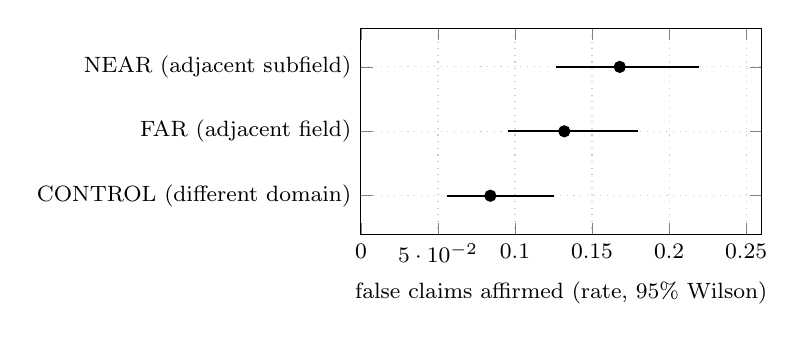
\begin{tikzpicture}
\begin{axis}[width=0.55\linewidth,height=4.2cm,xlabel={false claims affirmed (rate, 95\% Wilson)},xmin=0,xmax=0.26,ytick={1,2,3},yticklabels={NEAR (adjacent subfield),FAR (adjacent field),CONTROL (different domain)},ymin=0.4,ymax=3.6,y dir=reverse,grid=major,major grid style={dotted,gray!40},tick label style={font=\footnotesize},label style={font=\footnotesize}]
\addplot[black,thick] coordinates {(0.1268,1) (0.2193,1)};
\addplot[only marks,mark=*,black] coordinates {(0.1680,1)};
\addplot[black,thick] coordinates {(0.0956,2) (0.1796,2)};
\addplot[only marks,mark=*,black] coordinates {(0.1320,2)};
\addplot[black,thick] coordinates {(0.0556,3) (0.1250,3)};
\addplot[only marks,mark=*,black] coordinates {(0.0840,3)};
\end{axis}
\end{tikzpicture}

\caption{False-claim affirmation rates with 95\% Wilson intervals ($n=\tiNearN{}$ per stratum, drawn once).}
\label{fig:forest}
\end{figure}

\paragraph{False affirmations across semantic distance.}
Table~\ref{tab:e1} and Figure~\ref{fig:forest} summarize the confirmatory expertise audit. On attested claims, the endpoint confirms \tiAttRate{} ($[\tiAttLo{},\tiAttHi{}]$, \tiAttK{}/\tiAttN{}) in the main run and \tiCtlAttRate{} ($[\tiCtlAttLo{},\tiCtlAttHi{}]$, \tiCtlAttK{}/\tiCtlAttN{}) in the control run; all \tiAttMiss{} main-run and \tiCtlAttMiss{} control-run unparseable outputs occurred on attested claims, with zero explicit denials. Because the endpoint denies most false claims across all three negative strata, discrimination resides in the contrast between polarities rather than in the attested confirmation rate alone.

On constructed-false claims verified against each author's full \texttt{/works} record, the endpoint affirms \tiNearRate{} ($[\tiNearLo{},\tiNearHi{}]$, \tiNearK{}/\tiNearN{}) for NEAR (adjacent subfield), \tiFarRate{} ($[\tiFarLo{},\tiFarHi{}]$, \tiFarK{}/\tiFarN{}) for FAR (adjacent field), and \tiCtlRate{} ($[\tiCtlLo{},\tiCtlHi{}]$, \tiCtlK{}/\tiCtlN{}) for CONTROL (different domain). Pairwise Newcombe 95\% difference intervals resolve only the extremes: NEAR exceeds CONTROL by \tiNearCtlDiff{} ($[\tiNearCtlDiffLo{},\tiNearCtlDiffHi{}]$, a \tiRatioNearCtl{}$\times$ ratio), whereas FAR minus CONTROL (\tiFarCtlDiff{}, $[\tiFarCtlDiffLo{},\tiFarCtlDiffHi{}]$) and NEAR minus FAR (\tiNearFarDiff{}, $[\tiNearFarDiffLo{},\tiNearFarDiffHi{}]$) both span zero.

Post hoc, we evaluate the ordered gradient across the three false strata (\tiNearK{}/\tiNearN{}, \tiFarK{}/\tiFarN{}, \tiCtlK{}/\tiCtlN{}). Under an independence assumption, Pearson's homogeneity test gives $\chi^2 = \tiPostChiSq{}$ ($df=2$, $p = \tiPostChiP{}$), the Cochran--Armitage linear trend test with equal scores $(2, 1, 0)$ yields $z = \tiPostTrendZ{}$ ($p = \tiPostTrendP{}$), and a two-sided Fisher's exact test comparing NEAR against CONTROL gives $p = \tiPostFisherNcP{}$ (odds ratio \tiPostFisherNcOr{}). Comparing the two attested arms across runs (\tiAttK{}/\tiAttN{} vs.\ \tiCtlAttK{}/\tiCtlAttN{}) yields a Newcombe difference of \tiPostAttDiff{} ($[\tiPostAttDiffLo{},\tiPostAttDiffHi{}]$, Fisher $p = \tiPostAttFisherP{}$). Although the baseline shift does not reach significance, NEAR/FAR and CONTROL come from separate, unpaired runs; these tests quantify sampling variation only and do not substitute for a paired within-author draw (\S\ref{sec:limits}).

\paragraph{Row-level inspection of the control arm.}
The CONTROL stratum was added post hoc to test whether affirmations vanish when the false topic lies in a wholly different domain. Because \tiCtlK{} of \tiCtlN{} different-domain claims were affirmed, we conducted an unblinded, single-reader inspection of the cached evidence strings behind all \tiCtlK{} affirmations (committed as a structured artifact so it can be audited). Exactly \tiRdBroad{} involve generic topic labels supporting a loose topical match; \tiRdSame{} cite work in the claimed topic attributed to a same-name person or the same institution absent from the author's OpenAlex profile (consistent with a split profile, homonym, or classifier gap); and \tiRdOther{} name a different person, supply an unattributed title, or fail to support the topic altogether. Only the final group represents unambiguous endpoint error: \tiRdErrK{} of \tiRdErrN{} (\tiRdErrRate{}, 95\% Wilson $[\tiRdErrLo{},\tiRdErrHi{}]$). The control arm therefore does not operate as a pure negative control~\citep{lipsitch2010negative} and does not establish a strict error floor beneath NEAR and FAR.

\begin{table}[!tb]
\centering\small
\begin{tabular}{@{}lrlr@{}}
\toprule
Affirmed claim & $n$ & Cites a work by that author & No title resolvable \\
\midrule
Attested & 150 & 0.5733 [0.4933, 0.6497] & 49 (32.7\%) \\
False, adjacent field & 102 & 0.2843 [0.2058, 0.3784] & 56 (54.9\%) \\
False, adjacent subfield & 126 & 0.2302 [0.1653, 0.3110] & 73 (57.9\%) \\
False, different domain & 21 & 0.0000 [0.0000, 0.1546] & 14 (66.7\%) \\
\bottomrule
\end{tabular}

\caption{Citation-grounding audit across \tiAaTotal{} cached affirmations (\$0 API spend). A cited title that OpenAlex could not resolve counts as not backed; the final column shows the unresolvable-title share.}
\label{tab:a12}
\end{table}

\paragraph{Citation grounding.}
\label{sec:a12}
At zero additional API spend, we resolved up to three cited titles per affirmation against OpenAlex for \tiAaTotal{} cached affirmations: all \tiAaCtlN{} CONTROL affirmations, all false affirmations across both the confirmatory main run (\tiAaFarMain{} FAR, \tiAaNearMain{} NEAR) and the earlier contaminated run (\tiAaFarRaw{} FAR, \tiAaNearRaw{} NEAR), and \tiAaAttN{} of \tiAaAttAvail{} attested affirmations (Table~\ref{tab:a12}). Attested affirmations cite a verifiable work by the target author \tiAaAttRate{} of the time, adjacent false affirmations do so roughly a quarter of the time (\tiAaNearRate{} NEAR, \tiAaFarRate{} FAR), and CONTROL affirmations never (\tiAaCtlRate{}, $0/\tiAaCtlN{}$). Because ``backed'' requires only any real work by the author (even on another topic), because the adjacent rows pool in affirmations from the contaminated run, and because \tiAaAttNoTitleShare{}\% to \tiAaCtlNoTitleShare{}\% of affirmations contained no OpenAlex-resolvable title, Table~\ref{tab:a12} acts as an upper bound on author-level grounding rather than an independent oracle test.

\begin{figure}[!tb]
\centering
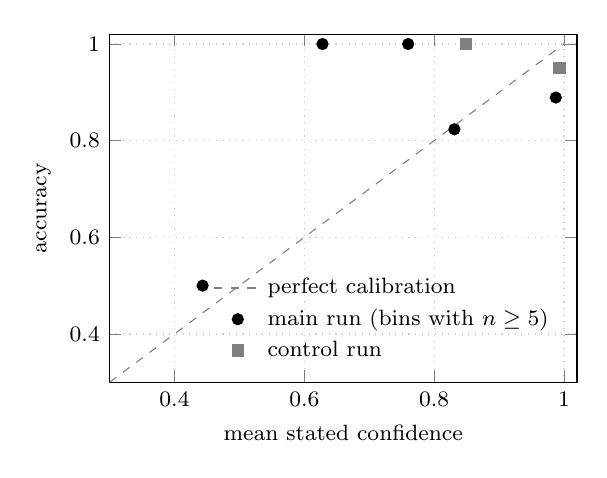
\begin{tikzpicture}
\begin{axis}[width=0.62\linewidth,height=6cm,xlabel={mean stated confidence},ylabel={accuracy},xmin=0.3,xmax=1.02,ymin=0.3,ymax=1.02,legend pos=south east,legend cell align=left,legend style={font=\footnotesize,draw=none,fill=none},grid=major,major grid style={dotted,gray!40},tick label style={font=\footnotesize},label style={font=\footnotesize}]
\addplot[gray,dashed] coordinates {(0.3,0.3) (1.0,1.0)};
\addlegendentry{perfect calibration}
\addplot[only marks,mark=*,black] coordinates {(0.0000,0.8750) (0.2400,1.0000) (0.4433,0.5000) (0.6280,1.0000) (0.7600,1.0000) (0.8312,0.8235) (0.9874,0.8892)};
\addlegendentry{main run (bins with $n \ge 5$)}
\addplot[only marks,mark=square*,gray] coordinates {(0.0000,0.8333) (0.8486,1.0000) (0.9930,0.9500)};
\addlegendentry{control run}
\end{axis}
\end{tikzpicture}

\caption{Reliability diagram for schema-elicited confidence (bins with $n \ge 5$). In the main run, \tiCalTopN{} of \tiCalN{} answers sit in the top $[0.9, 1.0]$ bin.}
\label{fig:rel}
\end{figure}

\begin{table}[!tb]
\centering\small
\begin{tabular}{@{}lrrrrrrr@{}}
\toprule
Run (task mix) & $n$ & Brier & Constant & Rel. & Res. & Resid. & BSS \\
\midrule
Main (1/3 attested, 2/3 false) & 750 & 0.1191 & 0.1005 & 0.0244 & 0.0024 & $-$0.0034 & $-$0.1852 \\
Control (1/2 attested, 1/2 false) & 500 & 0.0604 & 0.0475 & 0.0136 & 0.0002 & $-$0.0004 & $-$0.2716 \\
\bottomrule
\end{tabular}

\caption{Post-hoc Murphy (1973) 10-bin Brier score decomposition across both expertise runs. Constant denotes the hindsight base-rate Brier score (Uncertainty, $\bar{y}(1-\bar{y})$); Rel.\ is reliability (miscalibration penalty); Res.\ is bin resolution; Resid.\ is exact minus binned Brier; BSS $= 1 - \text{Brier}/\text{Constant}$.}
\label{tab:brier}
\end{table}

\paragraph{Stated confidence and Murphy Brier decomposition.}
Schema-elicited confidence sits pinned near ceiling (Figure~\ref{fig:rel}). In the main run, \tiCalTopN{} of \tiCalN{} answers (\tiCalTopShare{}\%) fall into $[0.9, 1.0]$ with mean confidence \tiCalTopConf{} against accuracy \tiCalTopAcc{} (a \tiCalTopGap{}-point overconfidence gap), producing ECE \tiEce{} and Brier score \tiBrier{}. Against a hindsight constant forecaster predicting the pooled main-run accuracy (\tiCalAccAll{}), whose Brier score is \tiBrierBase{}, the endpoint's confidence is strictly worse. The control run (50/50 polarity mix) exhibits the same ceiling pattern: \tiCtlCalTopN{} of \tiCtlCalN{} answers land in $[0.9, 1.0]$ at mean confidence \tiCtlCalTopConf{} against accuracy \tiCtlCalTopAcc{} (\tiCtlEmptyBins{} empty bins, ECE \tiCtlEce{}, Brier \tiCtlBrier{} vs.\ constant \tiPostCtlUnc{}).

Post hoc, Table~\ref{tab:brier} decomposes both Brier scores into Murphy's~\citep{murphy1973brier} reliability, resolution, and uncertainty components across the committed 10-bin summaries. In both task mixes, the Brier Skill Score is substantially negative (\tiPostMainBss{} main; \tiPostCtlBss{} control), and the miscalibration penalty (reliability: \tiPostMainRel{} main, \tiPostCtlRel{} control) exceeds bin resolution (\tiPostMainRes{} main, \tiPostCtlRes{} control) by more than an order of magnitude. The stated confidence carries negligible discriminative signal once answers concentrate at ceiling.

\section{Employment-surface pre-registered tests}
\label{sec:employment}

Three pre-registered employment-surface tests on SEC Section 16 filers completed on Exa \texttt{/answer}. Outcomes of all remaining registered arms appear in Appendix~\ref{app:prereg}.

\begin{table}[!tb]
\centering\small
\begin{tabular}{@{}lrrrl@{}}
\toprule
Band & A: name & C: + employer & D: + full anchor & Paired C $-$ A, 95\% bootstrap \\
\midrule
unique & 0.2375 & 0.3500 & 0.4625 & +0.1125 [+0.0250, +0.2000] \\
low (2--3) & 0.0500 & 0.2000 & 0.3375 & +0.1500 [+0.0750, +0.2375] \\
medium (4--9) & 0.0000 & 0.1875 & 0.2750 & +0.1875 [+0.1000, +0.2750] \\
high ($\ge$10) & 0.0000 & 0.2875 & 0.3000 & +0.2875 [+0.1875, +0.3875] \\
\bottomrule
\end{tabular}

\caption{E2: correct-identity rate by name-collision band and query rendering ($n=\tiEtwoN{}$ per band, seed \tiEtwoSeed{}). Arm C adds the past employer in free text; Arm D adds attested date and role. Paired differences are within task (10,000 bootstrap resamples).}
\label{tab:e2}
\end{table}

\paragraph{E2: Free-text employer context disambiguates colliding names.}
We pre-registered the hypothesis (motivated by structured-filter people indexes) that supplying a biographical constraint would not improve identity resolution over a bare name. On Exa \texttt{/answer}, that hypothesis is falsified (Table~\ref{tab:e2}). Name alone resolved \tiEtwoMAK{} of \tiEtwoMAN{} tasks in the medium collision band and \tiEtwoHAK{} of \tiEtwoHAN{} in the high band. Adding the past employer in free text (Arm C) lifted correct resolution across all four bands, with paired 95\% bootstrap intervals excluding zero in every band. Adding the attested filing date and role class (Arm D vs.\ C) yielded no measurable gain once names collided at medium or high degree. Because colliding bands are stratified rather than randomly sampled, rates describe band performance rather than population incidence, and the result scopes to free-text answer engines rather than structured-filter indexes.

\begin{table}[!tb]
\centering\small
\begin{tabular}{@{}lrrl@{}}
\toprule
Collision degree & $n$ & Wrong identity & Rate, 95\% Wilson \\
\midrule
1 (unique) & 80 & 3 & 0.0375 [0.0128, 0.1045] \\
2--3 & 80 & 0 & 0.0000 [0.0000, 0.0458] \\
4--9 & 80 & 1 & 0.0125 [0.0022, 0.0675] \\
$\ge$10 & 80 & 0 & 0.0000 [0.0000, 0.0458] \\
\bottomrule
\end{tabular}

\caption{H2: wrong-identity (\texttt{FALSE\_MERGE}) rate of the full-context arm by name-collision degree.}
\label{tab:h2}
\end{table}

\paragraph{H2: False merges do not rise with collision degree.}
Hypothesis H2 predicted that confidently wrong identity merges would increase with name-collision degree $d$. Evaluated at zero extra cost over E2's stratified draw (Table~\ref{tab:h2}), wrong-identity counts are \tiHtwoUK{}, \tiHtwoLK{}, \tiHtwoMK{}, and \tiHtwoHK{} out of \tiHtwoUN{} across the unique, low, medium, and high bands. Intervals overlap across bands, showing no rise with collision (and not establishing a decrease). Inspection of resolution reasons explains the mechanism: on colliding names, the endpoint usually fails to identify a resolvable individual and scores \texttt{MISS}, preventing a confident wrong merge.

\begin{figure}[!tb]
\centering
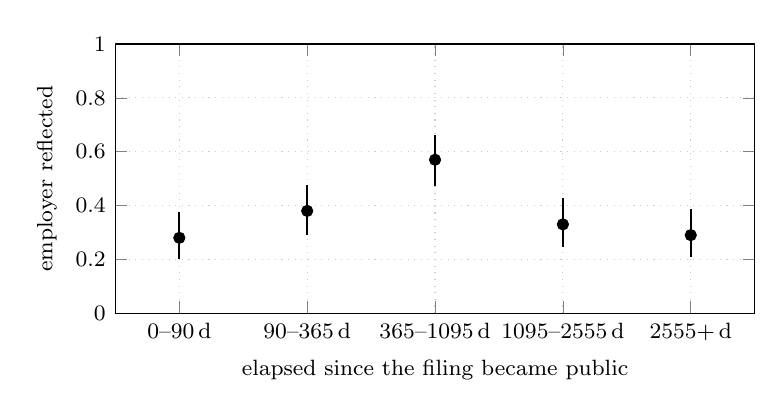
\begin{tikzpicture}
\begin{axis}[width=0.8\linewidth,height=5cm,xlabel={elapsed since the filing became public},ylabel={employer reflected},xtick={1,2,3,4,5},xticklabels={0--90\,d,90--365\,d,365--1095\,d,1095--2555\,d,2555+\,d},ymin=0,ymax=1,xmin=0.5,xmax=5.5,grid=major,major grid style={dotted,gray!40},tick label style={font=\footnotesize},label style={font=\footnotesize}]
\addplot[black,thick] coordinates {(1,0.2014) (1,0.3749)};
\addplot[black,thick] coordinates {(2,0.2910) (2,0.4779)};
\addplot[black,thick] coordinates {(3,0.4722) (3,0.6627)};
\addplot[black,thick] coordinates {(4,0.2456) (4,0.4269)};
\addplot[black,thick] coordinates {(5,0.2101) (5,0.3854)};
\addplot[only marks,mark=*,black] coordinates {(1,0.2800) (2,0.3800) (3,0.5700) (4,0.3300) (5,0.2900)};
\end{axis}
\end{tikzpicture}

\caption{H1: share of SEC filings whose attested employer was reflected by the endpoint, by elapsed time since filing ($n=100$ per bin, 95\% Wilson intervals).}
\label{fig:h1}
\end{figure}

\begin{table}[!tb]
\centering\small
\begin{tabular}{@{}lrl@{}}
\toprule
Elapsed since filing & $n$ & Reflected, 95\% Wilson \\
\midrule
0-90 d & 100 & 0.2800 [0.2014, 0.3749] \\
90-365 d & 100 & 0.3800 [0.2910, 0.4779] \\
365-1095 d & 100 & 0.5700 [0.4722, 0.6627] \\
1095-2555 d & 100 & 0.3300 [0.2456, 0.4269] \\
2555+ d & 100 & 0.2900 [0.2101, 0.3854] \\
\bottomrule
\end{tabular}

\caption{Binned reflection rates underlying Figure~\ref{fig:h1}.}
\label{tab:h1}
\end{table}

\paragraph{H1: Job-change reflection is non-monotone.}
Cross-sectional reflection of an attested employer change rises over the first three years after a filing and then declines beyond three years (Figure~\ref{fig:h1}, Table~\ref{tab:h1}). The late decline plausibly reflects executives moving again after the filing date (oracle ageing) rather than index regression. Because reflection is non-monotone, no unique half-life exists and the pre-registered survival hypothesis is mis-specified.

\section{Measurement failure modes caught by row-level inspection}
\label{sec:defects}

Automated API benchmarks interpose five software layers between a research question and a reported metric: query rendering, API filtering, response parsing, negative-example construction, and statistical summarization. Across the development of \texttt{titer}, each layer produced an aggregate failure that was indistinguishable in summary tables from a property of the system under evaluation. Table~\ref{tab:defects} catalogues these five failure modes, the spurious metrics they generated, the inspection step that exposed each defect, and the preventative gate.

\begin{table}[!tb]
\centering\footnotesize
\begin{tabularx}{\linewidth}{@{}l>{\raggedright\arraybackslash}p{2.3cm}>{\raggedright\arraybackslash}p{2.2cm}>{\raggedright\arraybackslash}X>{\raggedright\arraybackslash}p{2.6cm}@{}}
\toprule
Layer & Spurious output & Defect mechanism & Row-level diagnostic & Preventative gate \\
\midrule
1. Wire format & \tiPRunOneCorrect{}/\tiPRunOneN{} correct (Provider P) & Employer packed into free-text query instead of documented structured filters. & Returned rows showed right names at eponymous small businesses. & Adapter test asserting documented filter fields; 1-row pilot. \\
2. API filtering & \tiPRunTwoCorrect{}/\tiPRunTwoN{} correct (Provider P) & Current-state company filter always returned the anchor employer on historical move tasks. & Single structured query returned the anchor employer at rank 1. & Unit test forbidding filters on the scored anchor fact. \\
3. Response parsing & \tiWebCorrect{}/\tiWebN{} correct (web baseline) & Entity parser extracted filing identifiers from web page titles (\tiWebNotInCorpus{}/\tiWebN{} absent from corpus). & Printing raw parsed entity strings before scoring. & Inspect 10 parsed outputs on pilot before full run. \\
4. Negative oracle & \tiRawFar{} FAR, \tiRawNear{} NEAR ($n=\tiRawN{}$) & False topics checked against OpenAlex top-$N$ summary rather than exhaustive \texttt{/works}; true papers scored false. & Reading evidence strings revealed genuine co-authored papers. & Exhaustive \texttt{/works} check and catch-all exclusion (tested). \\
5. Summarization & Median lag \tiHoneIsoLag{} days (H1) & Isotonic regression forced monotonicity onto a rise-and-fall reflection curve. & Plotting binned empirical Wilson rates beneath the fitted curve. & Plot binned rates with CIs prior to shape-constrained fits. \\
\bottomrule
\end{tabularx}
\caption{Five measurement failure modes encountered during automated evaluation, each invisible in summary metrics alone. Provider P denotes the unmeasured structured-filter people index (Appendix~\ref{app:prereg}).}
\label{tab:defects}
\end{table}

\paragraph{The diagnostic principle.}
Aggregate accuracy cannot separate a defective measurement layer from an underperforming API: zero correct answers looks identical whether a record is absent or a wire format is wrong, and a \tiRawNear{} affirmation rate looks identical whether negatives are contaminated or the endpoint hallucinates. Two lightweight operational practices caught all five defects before publication: (i) executing a single-task or small-pilot call and reading the raw API payload and parsed fields verbatim before committing evaluation budget, and (ii) plotting binned empirical proportions with confidence intervals before fitting any shape-constrained estimator. Where possible, we encoded these lessons into automated regression tests (verifying structured filter usage, anchor exclusion, and exhaustive \texttt{/works} negative checks), though row-level inspection of new task surfaces remains an irreducible manual step.

\section{Limitations}
\label{sec:limits}

\begin{itemize}\setlength\itemsep{2pt}\setlength\parskip{0pt}
\item \textbf{One endpoint, one prompt, one schema, one draw.} Every surviving empirical number describes Exa \texttt{/answer} called with a single prompt wording and JSON \texttt{outputSchema}, queried once per task in September 2026 (seed \tiSeed{}) with unpinned backend model parameters. Prompt wording sensitivity~\citep{sclar2023prompt,mizrahi2023state}, sycophantic framing effects~\citep{sharma2023sycophancy}, and stochastic run-to-run variation (test--retest stability) were not measured.
\item \textbf{Unpaired cross-run distance gradient.} NEAR and FAR come from the main run and CONTROL from a separate post-hoc run drawn independently from a smaller author pool whose attested confirmation rate was higher (\tiCtlAttRate{} vs.\ \tiAttRate{}). The pairwise Newcombe intervals and post-hoc $\chi^2$, Cochran--Armitage, and Fisher tests treat strata as independent and do not account for cross-run variance.
\item \textbf{Oracle error and uncalibrated control floor.} OpenAlex topics come from a third-party ML classifier attached to single author profiles; split profiles, homonyms, unindexed works, and broad topic labels can turn a constructed negative into a valid match. Because an unblinded single-reader pass found only \tiRdOther{} of \tiCtlK{} CONTROL affirmations (\tiRdErrRate{}) clearly attributable to endpoint error, the control arm does not bound prompt-interpretation or oracle-error objections. The NEAR and FAR rates are therefore upper bounds carrying an unquantified oracle-error component; a random spot check of \tiSpotN{} negatives found zero contamination (upper bound \tiSpotHiPct{}\%), but affirmed claims selectively enrich for profile splits and classifier blind spots. Additionally, publication history is narrower than applied expertise.
\item \textbf{Population skew and calibration task mix.} ORCID-linked researchers (\tiAuthors{}) and SEC Section 16 filers (\tiCorpusPeople{}; \tiUsablePct{}\%, \tiUsableN{} usable tasks after four narrowings) have unusually high public web visibility, so error rates may not generalize to less-documented populations. Calibration summaries (ECE, Brier, Murphy components) depend on our schema-elicited confidence and balanced stratum mix (1/3 attested in the main run, 1/2 in the control run), with unparsed responses scored at confidence $0$.
\item \textbf{Endpoint scope and vendor coverage.} Exa \texttt{/answer} is a general question-answering API rather than a dedicated expertise verifier or people-search index. The Provider P structured-index arm remained unmeasured (Appendix~\ref{app:prereg}), and other commercial providers were excluded by Terms of Service reviewed on 2 September 2026.
\item \textbf{Terms of Service and vendor right-of-reply.} Section 4.2(a) of Exa's self-serve Terms (read 2 September and 23 November 2026) restricts publishing information obtained through the service; we report aggregate rates only with no record-level outputs and signed no Order Form or MSA. Resolving that clause formally and offering the vendor a documented right-of-reply remain open gates before any peer-reviewed venue submission.
\item \textbf{Reproducibility boundary.} Committed JSON artifacts regenerate every table, figure, and test in this paper. Raw API responses and named person--false-claim pairs are withheld under repository privacy and ethics rules, so live re-execution requires a new paid draw (roughly \$\tiEoneSpend{} for the main strata) against a potentially updated endpoint.
\end{itemize}

\section{Conclusion}
\label{sec:conclusion}

Auditing Exa \texttt{/answer} against OpenAlex authorship records and SEC Section 16 filings yields a clear empirical profile alongside a methodological caution. On expertise verification, the endpoint confirms \tiAttRate{} of attested claims while affirming \tiNearRate{} of adjacent-subfield, \tiFarRate{} of adjacent-field, and \tiCtlRate{} of different-domain unattested claims, with schema-elicited confidence pinned at ceiling and scoring worse than a constant base-rate forecast across both task mixes (Brier \tiBrier{} vs.\ \tiBrierBase{} main; \tiCtlBrier{} vs.\ \tiPostCtlUnc{} control). On SEC filings, free-text employer context substantially improves resolution of colliding names, false merges do not rise with collision degree, and job-change reflection is non-monotone. Simultaneously, five harness failure modes encountered during construction underscore that aggregate benchmark scores remain uninterpretable until raw returned rows and binned rates are inspected.

Closing the remaining threats to validity requires new API spend, independent human readers, and vendor engagement, all specified in the repository's v2 protocol (\texttt{docs/DESIGN-V2.md}): test--retest repeats on the \tiTotalCalls{} tasks, a blind two-reader adjudication over all 75 NEAR and FAR affirmations (plus the \tiCtlK{} CONTROL affirmations), a 2--4 prompt wording sweep, a paired within-author draw across all three negative distances, evaluation of a second answer endpoint alongside Provider P at its registered sample size ($n=\tiPowerN{}$ per arm), and legal review of Terms \S4.2(a) with a formal vendor right-of-reply prior to venue submission.

\section*{Disclosures and availability}

The code, analysis scripts, and manuscript were drafted with an AI coding assistant under the author's direction and review. The author works at a commercial AI gateway company; nothing from that product, its customers, or its internal data is used here. All inputs derive from public records or synthetic tests, and all API measurements used self-serve accounts with no vendor funding, review, or enterprise agreement. Exa has not yet been sent these results or offered a right of reply; resolving self-serve Terms \S4.2(a) and offering a vendor reply are explicit pre-venue gates (\S\ref{sec:limits}). Constructed-false claims are test inputs only and are never published paired with named individuals; any individual in the public-record corpora may request removal.

Repository work began on 2 September 2026 (first commit \texttt{fad6dc8}); the first preprint version (\texttt{paper-v1.0}, Zenodo record 24454863) was compiled on 23 November 2026, and this revision (\texttt{paper-v2.0}) is of 23 November 2026. Code and results are released under the MIT licence and this paper under CC BY 4.0. Repository: \url{https://github.com/caiotheodoro/titer}. Public pointer datasets (CC0): \url{https://huggingface.co/datasets/caiotheodoro/titer-edgar-officers} and \url{https://huggingface.co/datasets/caiotheodoro/titer-expertise-claims}.

\bibliographystyle{plainnat}
{\footnotesize\setlength{\bibsep}{0pt}\bibliography{refs}}

\appendix

\section{Pre-registration outcomes, retractions, and audit record}
\label{app:prereg}

Two pre-registrations were hash-frozen prior to data collection: the SEC employment study (\texttt{docs/PRE-REGISTRATION.md}, frozen 2 September 2026, covering H1--H4) and the OpenAlex expertise study (\texttt{docs/PRE-REGISTRATION-EXPERTISE.md}, frozen 3 September 2026, covering E1--E4). Table~\ref{tab:prereg} summarizes the disposition of every registered hypothesis, control arm, and unmeasured comparison.

\begin{table}[!htb]
\centering\footnotesize
\begin{tabularx}{\linewidth}{@{}l>{\raggedright\arraybackslash}p{2.7cm}>{\raggedright\arraybackslash}p{2.3cm}>{\raggedright\arraybackslash}X@{}}
\toprule
Arm / ID & Registered question & Status & Disposition and key figures \\
\midrule
E1 & False expertise affirmation & Retracted (R002), re-run & Raw top-$N$ rates (\tiRawFar{}, \tiRawNear{}, $n=\tiRawN{}$) retracted. Confirmatory verified-negative rates: \tiNearRate{} NEAR, \tiFarRate{} FAR, \tiAttRate{} ATTESTED ($n=\tiNearN{}$ each; Table~\ref{tab:e1}). Collision-degree clause not tested in E1 draw. \\
CONTROL & Different-domain negative control & Post hoc & Added after main run: \tiCtlRate{} (\tiCtlK{}/\tiCtlN{}), control attested \tiCtlAttRate{}. Single-reader pass: \tiRdOther{}/\tiCtlK{} (\tiRdErrRate{}) clear endpoint error. \\
E2 & Capability constraint on colliding names & Falsified on answer API & Free-text past employer raised accuracy across all 4 bands (Table~\ref{tab:e2}); D029 remains untested on structured-filter indexes. \\
E3 & Confidence calibration & Measured & \tiCalTopShare{}\% in $[0.9, 1.0]$ (mean \tiCalTopConf{} vs.\ \tiCalTopAcc{}); ECE \tiEce{}, Brier \tiBrier{} vs.\ constant \tiBrierBase{} (Table~\ref{tab:brier}). \\
E4 & SEC vs.\ scholar coverage & No verdict & Committed artifact holds only 4/250 scored scholar rows (\texttt{NO VERDICT}); earlier unbacked prose figures withdrawn. \\
H1 & Job-change reflection half-life & Mis-specified & Non-monotone rise-and-fall curve (Figure~\ref{fig:h1}, Table~\ref{tab:h1}); Kaplan--Meier replaced by isotonic, then withdrawn after spurious \tiHoneIsoLag{}-day lag. \\
H2 & False merges rise with collision $d$ & Falsified & \tiHtwoUK{}, \tiHtwoLK{}, \tiHtwoMK{}, \tiHtwoHK{} of \tiHtwoUN{} across bands (Table~\ref{tab:h2}); overlapping intervals show no rise. \\
H3 & Free-signal calibration (SEC) & Superseded & Unfinished on SEC population; E3 measures calibration on the expertise arm. \\
H4 & Live budget-aware policy (8B/4B) & Unmeasured live & No live-provider agent evaluation; an exploratory 130-parameter simulator policy (\tiEnvObs{} cached observations) was trained in the repository and is not claimed as a live result. \\
Provider P & Structured people-search index & Retracted (R001), unmeasured & Eight harness query defects across five budgets (\tiPRunOneCorrect{}/\tiPRunOneN{}, \tiPRunTwoCorrect{}/\tiPRunTwoN{}, \tiPRunFourCorrect{}/\tiPRunFourN{}, \tiPRunArmCorrect{}/\tiPRunArmN{}); no vendor accuracy claimed. Registered power requires $n=\tiPowerN{}$/arm (\$\tiPowerCost{} at \$\tiPowerPrice{}/search). \\
Web floor & Trivial free web baseline & Withdrawn & Parser extracted names from page titles (\tiWebCorrect{}/\tiWebN{}, \tiWebNotInCorpus{} absent from corpus); never validly measured. \\
\bottomrule
\end{tabularx}
\caption{Complete ledger of pre-registered hypotheses, post-hoc arms, retractions, and unmeasured arms across both frozen registrations.}
\label{tab:prereg}
\end{table}

\paragraph{Retractions and audit trail.}
Two formal retractions are logged in \texttt{docs/RETRACTIONS.md}: R001 voided the initial Provider P arm after row inspection revealed free-text wire-format packing, and R002 voided raw E1 rates after evidence inspection revealed top-$N$ OpenAlex negative contamination. During manuscript preparation, a cold repository audit (recorded in \texttt{docs/DECISIONS.md}, D046) identified and corrected documentation discrepancies---withdrawing unbacked E4 scholar counts and unsourced third-party comparison numbers, refreshing stale measurement-card floors, disclosing that Table~\ref{tab:a12} pools retracted-run adjacent affirmations, clarifying that the control arm's attested and false draws were independent, and withdrawing earlier prose that treated the \tiCtlRate{} control rate as a strict error floor. Post-hoc statistical checks (unpaired trend tests and Murphy Brier decomposition) were logged in D049 prior to computation and recorded in D050.

\end{document}
